\documentclass[letterpaper, 10 pt, conference]{ieeeconf}

%\let\labelindent\relax
%\IEEEoverridecommandlockouts
%\overrideIEEEmargins

%floats and figures
\usepackage{graphics}
\usepackage[pdftex]{graphicx}
\usepackage[font={small}]{caption}
\usepackage{subcaption}
%\usepackage[center]{subfigure} %DONT USE BOTH SUBCAPTION AND SUBFIGURE
%\DeclareGraphicsExtensions{.pdf,.png,.jpg}
%\usepackage{overpic}
%\usepackage[rightcaption]{sidecap}
%\usepackage{pbox}

%Math Stuff
\usepackage{mathtools}
\usepackage{amsmath, amssymb, amscd}
%\usepackage{ wasysym } %special symbols
\usepackage{amsfonts}
\usepackage{mathptmx}       % selects Times Roman as basic font
\DeclareMathAlphabet{\mathcal}{OMS}{lmsy}{m}{n}
\DeclareSymbolFont{largesymbols}{OMX}{cmex}{m}{n}
\usepackage{algorithm}
\usepackage{algorithmicx}
%\usepackage{algorithm}
%\usepackage{algpseudocode}
% \usepackage[ruled,vlined,linesnumbered]{algorithm2e}
\usepackage{ textcomp } %for getting text tilde

%Table Stuff
\usepackage{array} %for table entries to be in center of cell
\usepackage{tabularx}
\usepackage{multicol}
\usepackage{multirow}

%DOCUMENT WIDE
\usepackage{times} % assumes new font selection scheme installed
\usepackage{xspace}
\usepackage[english]{babel} %for hyphenation rules
%\usepackage{flushend}%balance columns on last page
\usepackage{fixltx2e} %fix latex issue across versions
\usepackage{bm}
\usepackage{units}

\usepackage{makeidx}
% \usepackage{enumitem}
\usepackage[yyyymmdd,hhmmss]{datetime}
\usepackage[english]{babel}

%Bibliography and cross-ref
\makeatletter
\let\NAT@parse\undefined
\makeatother
\usepackage[numbers]{natbib}
\renewcommand{\bibfont}{\footnotesize}
% \usepackage{cite} %DONT USE NATBIB AND CITE TOGETHER

%hyperlinking
\usepackage{url}
\makeatletter
\g@addto@macro{\UrlBreaks}{\UrlOrds}
\makeatother
\usepackage{color}
\usepackage[usenames,dvipsnames, table]{xcolor}
\usepackage[pdfborder={0 0 0.5}]{hyperref}
\hypersetup{
    colorlinks=true,
    linkcolor=blue,
    citecolor=black,
    filecolor=cyan,
    urlcolor=blue
}


%=======U S E R  D E F I N E D  M A C R O S=======
% \newcommand{\bibhref}[2]{#2}
\newcommand{\todo}[1]{\textcolor{red}{[ToDo:#1]}}
\newcommand{\tocite}[1]{\textcolor{red}{[cite]}}
\newcommand{\ignore}[1]{}

% Usage:
% \figlabel{myfigure} creates \label{fig:myfigure}
% \figref{myfigure} references it
\newcommand{\figlabel}[1]{\label{fig:#1}}
\newcommand{\figref}[1]{Figure~\ref{fig:#1}}

% Usage:
% \seclabel{mysection} creates \label{sec:mysection}
% \secref{mysection} references it
\newcommand{\seclabel}[1]{\label{sec:#1}}
\newcommand{\secref}[1]{Section~\ref{sec:#1}}

% Usage:
% \tablabel{mytable} creates \label{tab:mytable}
% \tabref{mytable} references it
\newcommand{\tablabel}[1]{\label{tab:#1}}
\newcommand{\tabref}[1]{Table~\ref{tab:#1}}

% use this command instead of writing "da Vinci" so it's never split 
\newcommand{\davinci}{da~Vinci\xspace}


\usepackage{blindtext}

%===============================================================

\title{\LARGE \bf
Deep Segmentation of Surgical Robot Trajectories from Video 
}
% Pixels to Primitives (P2P)

\author{%
Adithyavairavan Murali, Animesh Garg, Sanjay Krishnan, Florian Pokorny, Ken Goldberg
%Authors are with the Department of Electrical Engineering and Computer Sciences, University of California at Berkeley, CA, USA.}
\thanks{$^{1}$EECS, University of California, Berkeley; {\{sanjaykrishnan, adithya\_murali\}@berkeley.edu}}%
\thanks{$^{2}$IEOR and EECS, University of California, Berkeley; {\{animesh.garg, goldberg\}@berkeley.edu}}%
}

\newcommand{\sys}{\textsf{DeepSeg}\xspace}

\begin{document}

\maketitle

\begin{abstract}
Segmentation is an important first step in analyzing long running robotic tasks. 
For reliable results, it is important to consider both visual and kinematic data, as visual data provides important information about the state of the workspace. 
Existing unsupervised segmentation methodologies are limited in the ways they can leverage visual data and rely on annotations or complete knowledge of all objects in the world. In this paper, we propose a framework that takes a step towards unsupervised segmentation of robotic demonstrations using raw video (i.e., pixel data). 
We identify key transition events in kinematic data, cluster transitions together using visual data, and then identify segments of the raw video corresponding to these clusters of transition events. 
The resulting video segments can be used to design error recovery actions, parameter tuning, action classification, 
and operator skill assessment. 
\todo{Our results on x suggest y}
\end{abstract} 

\section{Introduction}
Segmentation is often a first step when modeling trajectories of a human teleoperator executing a multistep task.
This approach has been applied in robot skill-learning \cite{calinon2010learning, kruger2010learning, konidaris2011robot}, generalization to novel initial conditions in Learning from Demonstrations \cite{Niekum2015}, and operator skill classification \cite{Reiley2009}.
Segmentation models fall into three broad categories: (1) dictionary-based, (2) label-based, and (3) unsupervised.
Dictionary-based approaches set a pre-defined vocabulary of primitives \emph{a priori} and decompose new trajectories in terms of the primitives.
Label-based approaches require annotation of examples segments, and learn a segmentation policy from examples.
Unsupervised methods assume some structure to the data, e.g., local linearity, and fit trajectories to this model grouping together locally similar points.
Unsupervised techniques can avoid time consuming labeling or dependence on a pre-defined set of primitives.

Increasingly, fixed camera video recordings accompany kinematic recordings of human teleoperation in a variety of datasets [cite].
Video can provide important information about the state of the environment and the relative orientation of the robot and other objects.
This information is crucial for segmentation that does not overfit to the robot's exact position and learns higher level task properties (i.e., the robot needs to contact an object).
While label- and dictionary-based approaches have been applied to segment multi-modal demonstrations\cite{DBLP:dblp_conf/wacv/LeaHV15,zappella2013surgical}, existing unsupervised approaches rely on hand tuned features (Krishnan et al. [cite]) or poses for all objects in the workspace via AR markers (Neikum et al. [cite]).
Leveraging raw visual data, i.e., pixels, for unsupervised segmentation is challenging due to the dimensionality and the featurization problem.

\begin{figure}[ht]
\centering
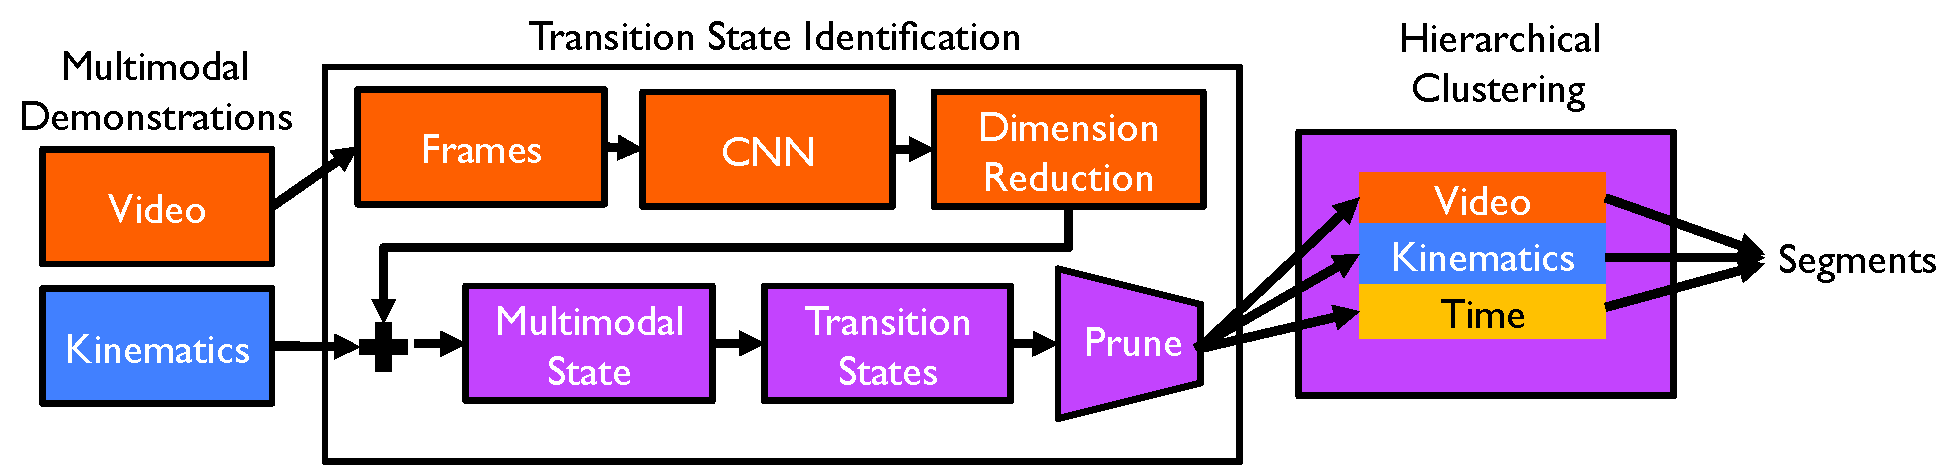
\includegraphics[width=\columnwidth]{figures/architecture.pdf}
\caption{\todo{name} architecture. We use a pre-trained CNN to featurize raw video data for use in segmentation. After featurization, we combine the data with kinematic data and apply a Transition State Clustering algorithm to identify segments. \label{fig:arch}}
\vspace{-1em}
\end{figure}

An application of particular interest is robotic surgery.
There are large and growing datasets of teleoperated surgical tasks with kinematic and camera recordings.
These recordings can facilitate automation via finite state machines, but a first step is segmentation.
In our prior work (Krishnan et al. [cite]), recognizing a number of surgery specific challenges such as temporal inconsistency and looping e.g., where a surgeon may attempt insertion 2-3 times, we proposed a non-parametric Bayesian model called Transition State Clustering (TSC).
Essentially, the model identifies states that mark linear dynamical regime transitions and clusters these states across demonstrations considering both spatial and temporal similarity.
Our results on real and synthetic data suggests this model is more robust to the demonstration inconsistencies prevalent in surgical tasks, even when these tasks were executed in a consistent environment (i.e., identical tissue phantoms). 

In this paper, we propose a \todo{name} algorithm that applies unsupervised segmentation to surgical demonstrations consisting of kinematic trajectories and video data.
To address the featurization problem in video, we leverage the growing maturity of Convolution Neural Networks (CNNs) in computer vision.
There are a number of architectures  (e.g., AlexNet [cite]) that are trained on immensely large datasets of nature images, and these pre-trained models can be applied to featurize video.
However, using a CNN as a featurizer is only part of the solution.
We design a variant of the TSC method to jointly consider both kinematic and high-dimensional featurized video data.
We illustrate the architecture in Figure \ref{fig:arch}.

In this application, pre-trained neural networks give us a convenient and transferable featurization.
We can leverage large datasets without having to do the training ourselves.
These results are complementary to the Bayesian model described in our prior work.
We model demonstrations as a time-varying stochastic process, with a discrete set of switching points.
At each time $t$, there is a hidden latent state that generates both the kinematics and video data.
Our goal is to define a segmentation w.r.t to that hidden state.
The algorithm that we propose in this paper is one approach to fit parameters to this model.

\todo{add about CCA if it pans out, add about fine tuning}

In summary, our contributions are as follows:
\begin{enumerate}
\item We propose an algorithm to segment demonstrations from kinematic and raw video data via a pre-trained CNN.
\item We describe a generative model to integrate the two types of data with dimensionality reduction.
\item We provide a comprehensive evaluation of parameters and model choice when using pre-trained CNNs for use with robotic demonstrations.
\item \todo{results suggest...}
\end{enumerate}


\section{Related Work}

\noindent\textbf{Surgical Segmentation: }

\begin{enumerate}
\item Describe ``surgeme" work
\end{enumerate}

\noindent\textbf{Segmentation in Other Robotics: }

\begin{enumerate}
\item Describe Neikum/others like DMP, GMM etc.
\end{enumerate}

\noindent\textbf{Related work in Computer Vision: }

\begin{enumerate}
\item Introduce Convolutional Network Research.
\end{enumerate}

\section{Problem Setup and Notation}

\subsection{High-level Problem}
\begin{enumerate}
\item Complex stochastic process involving video data and kinematic data.
\item Our hypothesis is when tasks are long running this stochastic process switches between simpler ``regimes".
\item Find a discrete parametrization for switching criteria. (Aka TSC)
\end{enumerate}

\subsection{Introduction to TSC}
\begin{enumerate}
\item Describe ISRR paper and some basic results
\end{enumerate}

\subsection{TSC in Visual Feature Space}

\begin{enumerate}
\item Describe a generative model top down that describes how all the variables are linked.
\end{enumerate}

\begin{figure}
\centering
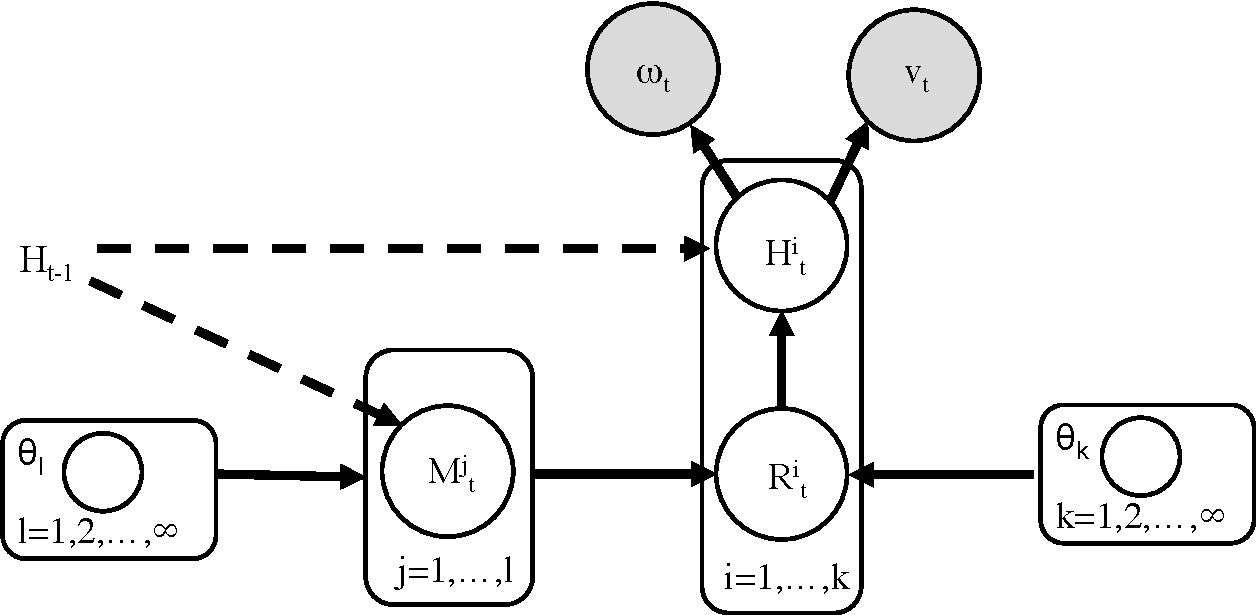
\includegraphics[width=\columnwidth]{figures/probabilistic_graphical_model.pdf}
\caption{We model the set of demonstrations as observations from a noisy stochastic process. Here we describe the graphical model for this process. There is a latent variable $H_t$ that links kinematic (shaded) and visual observations (shaded) and the \sys framework learns a discrete parametrization of this process (unshaded). }
\label{fig:pgm}
\end{figure}

\subsection{Overview of the Algorithm}
\begin{enumerate}
\item Describe the basic algorithm to learn the model and forward reference key components.
\end{enumerate}
\section{Visual Featurization}
\begin{enumerate}

\item Describe goals

\begin{enumerate}
\item Spatially \& Scale invariant features
\item Key in on primitives
\end{enumerate}

\item Describe different ways that you can get visual features
\begin{enumerate}
\item Deep features from Convolutional Neural Networks
\begin{enumerate}
\item Pre-trained Architectures (VGG, AlexNet, C3D)
\item Encoding
\item Dimensionality-reduction and Correlation
\end{enumerate}
\item Tracking with Optical Flow
\item HOG
\item SIFT
\item PCA on RGB Images LOL \\
Need to show Figure with PCA? on all of them 
\end{enumerate}

\item Describe what we did and our methodology

\item Pre-processing
\begin{itemize}
\item Background subtraction
\begin{itemize}
\item A OpenCV built-in background subtraction algorithm was applied on each frame before pushing through the CNN. The algorithm was a Gaussian Mixture-based Background/Foreground Segmentation algorithm. It was introduced in the paper "An improved adaptive background mixture model for real-time tracking with shadow detection" by P. KadewTraKuPong and R. Bowden in 2001.
\end{itemize}

\item Cropping \& Scaling
\begin{itemize}
\item I cropped all frames by equal amounts to capture only the workspace where most of the robot manipulation happened. Then, they were rescaled to 640 x 480 dimensions. All pre-processing happened with ffmpeg.
\end{itemize}

\end{itemize}


\end{enumerate}
\section{Latent State $H_t$}
Describe the process of linking kinematics and video (PCA, CCA, etc.).
If we apply any VLAD or encoding, or batching, describe it here:

\begin{itemize}
\item Encoding - Current Status
\begin{itemize}
\item So I've implemented the following encoding method- Latent Content Descriptors (LCD) + VLAD. However, initial results weren't great and I need to see how it performs on milestones clustering.
\end{itemize}

\item Temporal Batching - Current Status
\begin{itemize}
\item While batching is supposed to help in video analysis , I've seen good separation of clusters (PCA on conv features) with just individual frames without clustering... I think I need to look into this more and need to test it out with milestones clustering.
\end{itemize}

\end{itemize}

\section{Clustering}
Describe the clustering procedure--refer to ISRR when needed.

\section{Results}
\subsection{Exp1. End-to-end result with some task}

\begin{enumerate}
\item Show that clusters are sensible and align with some intuitive criteria e.g., surgemes
\end{enumerate}

\subsection{Exp2. Does Vision Help}

\begin{enumerate}
\item Remove visual features and show that clusters degrade
\end{enumerate}

\subsection{Exp3. Parameter Search}

\begin{enumerate}
\item Describe our eval procedure and how we arrived at the architecture we did.
\end{enumerate}

\subsection{Exp4. Robustness}
\item Add noise or corrupt images and test to see how robust the segmentations we learn are.
\end{enumerate}

\section{Conclusion}
Summarize framework and results.


\bibliographystyle{IEEEtranS}
\bibliography{library,palpationCASE}

\end{document}
